\documentclass{article}
\usepackage[margin=1in]{geometry}
\usepackage{amsmath,amsthm,amssymb}
\usepackage{bbm,enumerate,mathtools}
\usepackage{tikz,pgfplots}
\usepackage{chessboard}
\usepackage[hidelinks]{hyperref}
\usepackage{multicol} % Problem 35

\newenvironment{question}{\begin{trivlist}\item[\textbf{Question.}]}{\end{trivlist}}
\newenvironment{note}{\begin{trivlist}\item[\textbf{Note.}]}{\end{trivlist}}
\newenvironment{references}{\begin{trivlist}\item[\textbf{References.}]}{\end{trivlist}}
\newenvironment{related}{\begin{trivlist}\item[\textbf{Related.}]\end{trivlist}\begin{enumerate}}{\end{enumerate}}


\begin{document}
\rating{2}{2}
Ezgi showed me a puzzle where dominoes are placed to form a rectangle such that
there is no line that separates the dominoes into two rectangles.
\begin{figure}[ht!]
  \centering
  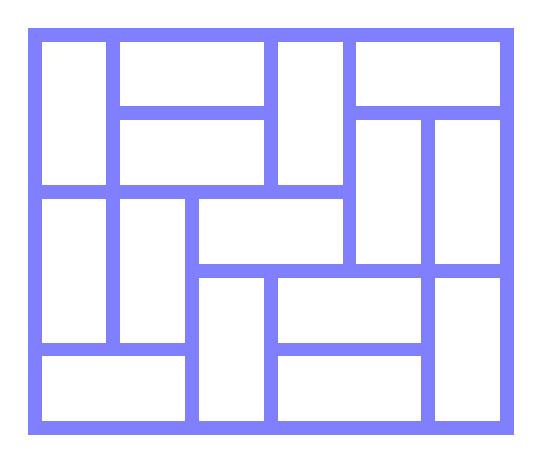
\begin{tikzpicture}[scale=1]
    \draw[blue!50, line width=5]
      (0,6) rectangle (1,4)
      (1,6) rectangle (3,5)
      (3,6) rectangle (4,4)
      (4,6) rectangle (6,5)
      (1,5) rectangle (3,4)
      (4,5) rectangle (5,3)
      (5,5) rectangle (6,3)
      (0,4) rectangle (1,2)
      (1,4) rectangle (2,2)
      (2,4) rectangle (4,3)
      (2,3) rectangle (3,1)
      (3,3) rectangle (5,2)
      (5,3) rectangle (6,1)
      (0,2) rectangle (2,1)
      (3,2) rectangle (5,1);
  \end{tikzpicture}
  \hspace{0.7cm}
  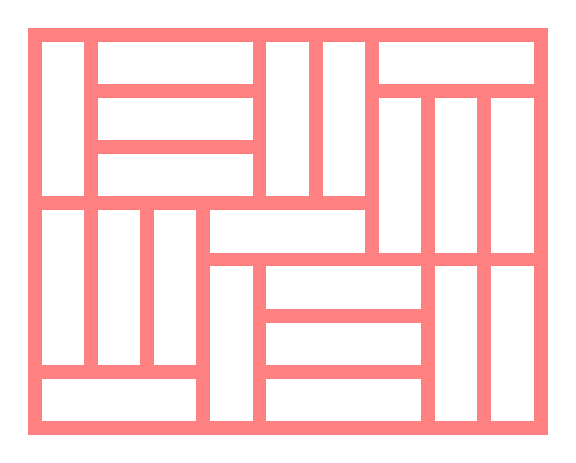
\begin{tikzpicture}[scale=0.714]
    \draw[red!50, line width=5]
      (0,0) rectangle (3,1)
      (0,1) rectangle (1,4)
      (0,4) rectangle (1,7)
      (1,1) rectangle (2,4)
      (1,4) rectangle (4,5)
      (1,5) rectangle (4,6)
      (1,6) rectangle (4,7)
      (2,1) rectangle (3,4)
      (3,0) rectangle (4,3)
      (3,3) rectangle (6,4)
      (4,0) rectangle (7,1)
      (4,1) rectangle (7,2)
      (4,2) rectangle (7,3)
      (4,4) rectangle (5,7)
      (5,4) rectangle (6,7)
      (6,3) rectangle (7,6)
      (6,6) rectangle (9,7)
      (7,0) rectangle (8,3)
      (7,3) rectangle (8,6)
      (8,0) rectangle (9,3)
      (8,3) rectangle (9,6);
  \end{tikzpicture}
  \caption{
    On the right is the smallest way to place dominoes into a rectangle such that there is no
    way to partition the dominoes into two rectangles.
    Is the left a minimal configuration with $1\times3$ triominoes?
  }
\end{figure}
\begin{question}
  What size grids have such configurations?
\end{question}

\begin{related}
  \item How many configurations exist for a given grid size?
  \item What if other rectangular polyominoes are used? (e.g. $3 \times 2$ hexominoes)
  \item Are there analogous problems for triangular grids? Higher dimensions?
\end{related}

\begin{note}
  These are sometimes called ``Fault-free domomino tilings''.
\end{note}

\begin{references}
  \item Project Euler, Problem 215.
  \item \url{http://mathworld.wolfram.com/Fault-FreeRectangle.html}
\end{references}
\end{document}
